\section{用折纸法画抛物线}
\markboth{1. 用折纸法画抛物线}{1. 用折纸法画抛物线}

高中的学生都知道，抛物线是与一个定点 $F$ 及一条定直线 $a$ 距离相等的点的轨迹。$F$ 叫做这条抛物线的焦点，$a$ 叫做它的准线。

抛物线用圆规直尺是作不出来的，可是用一张矩形的纸却可以“折出”一段抛物线。图 1.1 中，有一张矩形纸片，设它的一条边为准线 $a$。在纸片内部居中的地方取一个点 $F$ 作为焦点，用笔在 $F$ 的位置做上记号。然后把纸片折一次，使得 $a$ 边正好通过 $F$，或者说 $a$ 边上有一点与 $F$ 重合，然后抹平纸片，得到一条折痕 $l$（为了看得清楚，不妨用笔把直线 $l$ 描出来）。继续这样折下去，得到若干条折痕，你会发现这些折痕“围出”一条抛物线的轮廓（图 1.2）。只要画一条与这些折痕都相切的光滑曲线，就能得到所要画的抛物线了。

\begin{figure}[htbp]
  \centering
  \begin{minipage}[t]{0.47\textwidth}
    \centering
    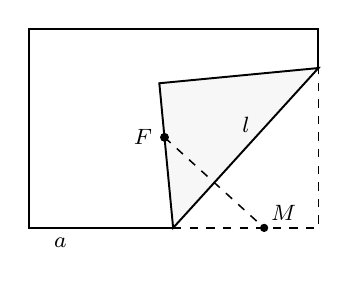
\begin{tikzpicture}[scale=1.15]
      % 矩形纸片范围: [0, 3.2] x [0, 2.2]
      % F = (1.5, 1.0), M = (2.6, 0)
      % 折痕 l 为 FM 的垂直平分线: 与 y=0 交于 A1=(1.5955, 0), 与 x=3.2 交于 A2=(3.2, 1.765)
      % 右下角 C=(3.2, 0) 关于 l 的对称点 C'=(1.443, 1.597)
      \coordinate (O) at (0,0);
      \coordinate (TL) at (0,2.2);
      \coordinate (TR) at (3.2,2.2);
      \coordinate (C) at (3.2,0);
      \coordinate (A1) at (1.5955,0);
      \coordinate (A2) at (3.2,1.765);
      \coordinate (Cp) at (1.443,1.597);
      \coordinate (F) at (1.5,1.0);
      \coordinate (M) at (2.6,0);

      % 原始纸片保留边
      \draw[line width=0.7pt] (A1) -- (O) -- (TL) -- (TR) -- (A2);
      % 原右下角虚线
      \draw[dashed, line width=0.6pt] (A1) -- (C) -- (A2);
      % 折起部分与折痕 l
      \draw[fill=gray!6, line width=0.7pt] (A1) -- (Cp) -- (A2) -- cycle;
      % 虚线 FM
      \draw[dashed, line width=0.55pt] (F) -- (M);

      % 标记点 F, M
      \fill (F) circle (1.4pt) node[left=1pt] {\footnotesize $F$};
      \fill (M) circle (1.3pt) node[above right=-1pt] {\footnotesize $M$};

      % 标注 a 与 l
      \node[below] at (0.35,0) {\footnotesize $a$};
      \node[above left] at (2.55,0.95) {\footnotesize $l$};
    \end{tikzpicture}
    \caption*{图\ 1.1}
  \end{minipage}
  \hfill
  \begin{minipage}[t]{0.47\textwidth}
    \centering
    \begin{tikzpicture}[scale=1.15]
      % 矩形 [0, 3.2] x [0, 2.2], F=(1.6, 0.9), a: y=0
      \draw[line width=0.7pt] (0,0) rectangle (3.2,2.2);
      \begin{scope}
        \clip (0,0) rectangle (3.2,2.2);
        % 绘制若干折痕: 对 m in [-0.2, 3.4], y = ((m-1.6)/0.9)*(x - (m+1.6)/2) + 0.45
        \foreach \m in {-0.2, 0.15, 0.5, 0.85, 1.2, 1.55, 1.9, 2.25, 2.6, 2.95, 3.3} {
          \pgfmathsetmacro{\ya}{((\m-1.6)/0.9)*(0 - (\m+1.6)/2) + 0.45}
          \pgfmathsetmacro{\yb}{((\m-1.6)/0.9)*(3.2 - (\m+1.6)/2) + 0.45}
          \draw[line width=0.45pt, black!80] (0,\ya) -- (3.2,\yb);
        }
        % 抛物线包络: y = (x-1.6)^2 / 1.8 + 0.45
        \draw[line width=0.9pt, curveblue, domain=0:3.2, samples=80]
          plot (\x, {(\x-1.6)*(\x-1.6)/1.8 + 0.45});
      \end{scope}
      \draw[fill=white, line width=0.7pt] (1.6,0.9) circle (1.5pt);
      \node[above] at (1.6,0.94) {\footnotesize $F$};
      \node[below] at (0.35,0) {\footnotesize $a$};
    \end{tikzpicture}
    \caption*{图\ 1.2}
  \end{minipage}
\end{figure}

\begin{center}
  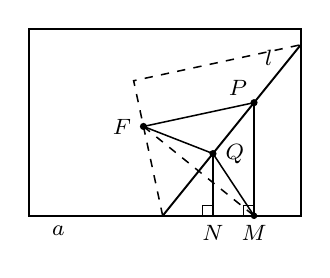
\begin{tikzpicture}[scale=1.08]
    % F = (1.35, 1.05), M = (2.65, 0)
    % 折痕 l 为 FM 中垂线: A1 = (1.57596, 0), A2 = (3.2, 2.01071)
    % 右下角 C = (3.2, 0) 关于 l 的精确对称点 C' = (1.23429, 1.58769)
    % 验证: A1, F, C' 严格共线, |A1 F| = |A1 M| = 1.07404, |F C'| = |M C| = 0.55
    \coordinate (O) at (0,0);
    \coordinate (TL) at (0,2.2);
    \coordinate (TR) at (3.2,2.2);
    \coordinate (C) at (3.2,0);
    \coordinate (A1) at (1.57596,0);
    \coordinate (A2) at (3.2,2.01071);
    \coordinate (Cp) at (1.23429,1.58769);
    \coordinate (F) at (1.35,1.05);
    \coordinate (M) at (2.65,0);
    \coordinate (P) at (2.65,1.32976);
    \coordinate (Q) at (2.167,0.7310);
    \coordinate (N) at (2.167,0);

    % 矩形纸片外框与折痕 l
    \draw[line width=0.7pt] (O) rectangle (TR);
    \draw[dashed, line width=0.55pt] (A1) -- (Cp) -- (A2);
    \draw[line width=0.7pt] (A1) -- (A2);

    % 辅助线段
    \draw[line width=0.55pt] (P) -- (M);
    \draw[line width=0.55pt] (Q) -- (N);
    \draw[dashed, line width=0.55pt] (F) -- (M);
    \draw[line width=0.55pt] (P) -- (F);
    \draw[line width=0.55pt] (Q) -- (F);
    \draw[line width=0.55pt] (Q) -- (M);

    % 直角符号
    \draw[line width=0.45pt] (M) ++(-0.12,0) -- ++(0,0.12) -- ++(0.12,0);
    \draw[line width=0.45pt] (N) ++(-0.12,0) -- ++(0,0.12) -- ++(0.12,0);

    % 点与标签
    \fill (F) circle (1.2pt) node[left=1pt] {\footnotesize $F$};
    \fill (P) circle (1.2pt) node[above left=-1pt] {\footnotesize $P$};
    \fill (Q) circle (1.2pt) node[right=1pt] {\footnotesize $Q$};
    \fill (M) circle (1.1pt) node[below] {\footnotesize $M$};
    \node[below] at (N) {\footnotesize $N$};
    \node[below] at (0.35,0) {\footnotesize $a$};
    \node[above left] at (2.98,1.65) {\footnotesize $l$};
  \end{tikzpicture}
  \par\vspace{4pt}{\footnotesize 图\ 1.3}
\end{center}

这种方法很有趣，要证明所得曲线确是抛物线也不难。如图 1.3，根据折法，直线 $a$ 上的点 $M$ 关于折痕 $l$ 与 $F$ 点对称。作 $MP \perp a$，交 $l$ 于 $P$；连 $PF$，则 $PF = PM$，即 $P$ 到定点 $F$ 的距离等于到定直线 $a$ 的距离，所以点 $P$ 在以 $F$ 为焦点、$a$ 为准线的抛物线上。其次，设 $Q$ 是 $l$ 上不同于 $P$ 的任意一点。连 $QF$、$QM$，作 $QN \perp a$，设垂足为 $N$，那么由直角三角形斜边大于直角边的性质，有
\[
  QF = QM > QN,
\]
总之，$QF \neq QN$，所以 $Q$ 点不在这条抛物线上。直线 $l$ 与这条抛物线有且只有一个公共点 $P$，并且由折纸方法知道 $l$ 不会垂直于 $a$，因而 $l$ 一定是这条抛物线的一条切线。同理，每条折痕都是这抛物线的一条切线。若干条折痕包围住同一条抛物线，就把这条抛物线的轮廓清楚地显示出来了。
